\def\W{6cm}
\def\H{2cm}
\begin{tikzpicture}[draw=black!50, node distance=0.3cm]
\pgfmathsetseed{99}
\tikzstyle{block}=[draw=none,rectangle,fill=none,inner sep=0pt]

\node[block] (s1) {\resizebox{0.1\linewidth}{!}{\begin{tikzpicture}
\begin{axis}[
	axis lines*=middle,
	enlargelimits = false,
	clip=false,
	scale only axis,
	hide y axis,
	width=0.5\textwidth,
	height=0.15\textwidth,
	ymin=-1.3,
	ymax=1.3,
	xmin=-11,
	xmax=11,
	axis line style={->,>=stealth},
	xlabel={\small $n$},
	every axis x label/.style={
		at={(ticklabel* cs:1)},
		xshift=0.2cm,
		anchor=north,
	},
	%xtick=\empty,
	ytick=\empty,
	xtick=\empty,
	%xtick={-3.14, -1, 1, 3.14},
	%xticklabels={$-\pi$, $-\omega_c$, $\omega_c$, $\pi$},
	%xmajorgrids,
	%ymajorgrids,
	every outer y axis line/.append style={white!15!black},
	every y tick label/.append style={font=\color{white!15!black}},
	legend style={draw=white!15!black,fill=white,legend cell align=left}]
	\addplot[ycomb, mark=*, fill=white, mark options={scale=0.75, fill=white}, line width=1pt, domain=-10:10, samples=21] {rand};
\end{axis}
\end{tikzpicture}
}};
\node[left=0cm of s1,scale=0.15] {$X(n, \chi_1)$};

\onslide<2->{
	\node[block, below of=s1] (s2) {\resizebox{0.1\linewidth}{!}{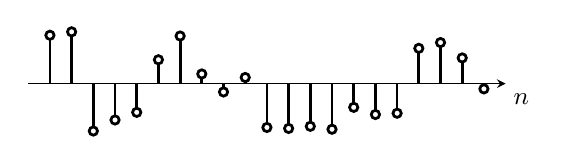
\begin{tikzpicture}
\begin{axis}[
	axis lines*=middle,
	enlargelimits = false,
	clip=false,
	scale only axis,
	hide y axis,
	width=0.5\textwidth,
	height=0.15\textwidth,
	ymin=-1.3,
	ymax=1.3,
	xmin=-11,
	xmax=11,
	axis line style={->,>=stealth},
	xlabel={\small $n$},
	every axis x label/.style={
		at={(ticklabel* cs:1)},
		xshift=0.2cm,
		anchor=north,
	},
	%xtick=\empty,
	ytick=\empty,
	xtick=\empty,
	%xtick={-3.14, -1, 1, 3.14},
	%xticklabels={$-\pi$, $-\omega_c$, $\omega_c$, $\pi$},
	%xmajorgrids,
	%ymajorgrids,
	every outer y axis line/.append style={white!15!black},
	every y tick label/.append style={font=\color{white!15!black}},
	legend style={draw=white!15!black,fill=white,legend cell align=left}]
	\addplot[ycomb, mark=*, fill=white, mark options={scale=0.75, fill=white}, line width=1pt, domain=-10:10, samples=21] {rand};
\end{axis}
\end{tikzpicture}
}};
	\node[left=0cm of s2,scale=0.15] {$X(n, \chi_2)$};
}

\onslide<3->{
	\node[block, below of=s2] (s3) {\resizebox{0.1\linewidth}{!}{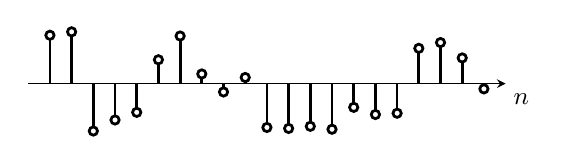
\begin{tikzpicture}
\begin{axis}[
	axis lines*=middle,
	enlargelimits = false,
	clip=false,
	scale only axis,
	hide y axis,
	width=0.5\textwidth,
	height=0.15\textwidth,
	ymin=-1.3,
	ymax=1.3,
	xmin=-11,
	xmax=11,
	axis line style={->,>=stealth},
	xlabel={\small $n$},
	every axis x label/.style={
		at={(ticklabel* cs:1)},
		xshift=0.2cm,
		anchor=north,
	},
	%xtick=\empty,
	ytick=\empty,
	xtick=\empty,
	%xtick={-3.14, -1, 1, 3.14},
	%xticklabels={$-\pi$, $-\omega_c$, $\omega_c$, $\pi$},
	%xmajorgrids,
	%ymajorgrids,
	every outer y axis line/.append style={white!15!black},
	every y tick label/.append style={font=\color{white!15!black}},
	legend style={draw=white!15!black,fill=white,legend cell align=left}]
	\addplot[ycomb, mark=*, fill=white, mark options={scale=0.75, fill=white}, line width=1pt, domain=-10:10, samples=21] {rand};
\end{axis}
\end{tikzpicture}
}};
	\node[left=0cm of s3,scale=0.15] {$X(n, \chi_3)$};
	\node[below=0cm of s3, scale=0.2] (dots) {\Large $\vdots$};
}

\onslide<4->{
\draw[red, very thin] ($(s1.north) + (-0.02,0)$) rectangle ($(dots.south) + (0.03,0)$);
\node [scale=0.15] (dist) at ($(s1.north) + (0.3cm, 0.05cm)$) {$x_n\sim p_{x_n}(x_n)$};
\draw [-{Latex[length=0.2mm,width=0.2mm]}, very thin, red,scale=0.1] (s1.north) to[out=90, in=180] (dist.west) (dist);
}

\onslide<5->{
\draw[red, very thin] ($(s1.north) + (-0.42,0)$) rectangle ($(dots.south) + (-0.38,0)$);
\node [scale=0.15] (dist2) at ($(s1.north) + (-0.12cm, 0.1cm)$) {$x_m\sim p_{x_m}(x_m)$};
\draw [-{Latex[length=0.2mm,width=0.2mm]}, very thin, red,scale=0.1] ($(s1.north) + (-4,0)$) to[out=90, in=180] (dist2.west);
}
\end{tikzpicture}

